\cotefile{53}
\scanpage{29}
% @ 1–4
d'un monoïde affine $G$, celà signifie aussi qu'il existe une opération de $G$ sur $M'$ \deleted{\unsure{qui}} telle que $M\unsure{-|\to}M'$ soit comp. avec \unsure{son|ses} op., et il est clair \inserted{\unsure{directemt}} (comme $W(M)\mathrel{-}W(M')$ \unsure{épi|épis}) que cette opération sera unique.

% @ 5–6
Si on a un mono
\[
M''\overset{i}{\hookrightarrow}M
\]
% @ 7–9
alors il ne sera pas vrai en général que $V(M)\mathrel{-}V(\unsure{M''|M'})$ soit surjectif, ni que $W(M'')\mathrel{-}W(M)$ soit injectif, donc \deleted{\unsure{faute de}} \unsure{cette|en tte} condition on \unsure{aura|a} du mal à parler d'opération induite.
% @ 10–12
\deleted{\unsure{Crt il est|Cert il est}} On dira qu'il \uline{existe} une op. induite si on peut faire opérer $G$ sur $M''$ de telle façon que $M''\mathrel{-}M$ soit comp. aux opérations.
% @ 13–15
Mais il n'est plus clair que l'op. ``induite'' soit unique ! En termes d'alg. comm., la question est de trouver un $\Delta_{M''}:M''\to M''\otimes A$ rendant commutatif
% @ 16–18 diagram
\diagram{\begin{tikzcd}[ampersand replacement=\&,row sep=large,column sep=large]
 M'' \arrow[r,dash,"{u_{M''}\,?}",to path={.. controls +(right:4mm) and +(left:4mm) .. (\tikztotarget) \tikztonodes -- ++(-.3pt,-1.4pt)}] \& M''\otimes A \arrow[d,dash,"{i\otimes{\mathrm{id}}_A}",to path={-- (\tikztotarget) \tikztonodes -- ++(.7pt,-1.2pt)}] \\
 M \arrow[u,dash,"i"',to path={-- (\tikztotarget) \tikztonodes .. controls +(up:2pt) and +(up:1pt) .. ++(2.5pt,.2pt)}] \arrow[r,dash,"{u_M}",to path={-- (\tikztotarget) \tikztonodes -- ++(0pt,1.1pt)}] \& M\otimes A
\end{tikzcd}}

% @ 19–20
On peut dire que c'est uniquement déterminé pourvu que $i\otimes{\mathrm{id}}_A=i_A$ soit un mono,
% @ 20 interlinear
\inserted{et si $\unsure{i|j}\otimes{\mathrm{id}}_{A\otimes A}$ l'est aussi, alors la condition $u_M(M'')\subset\mathrm{Im}\,M''_{\otimes A}$ est néc. et \uline{suffisante} pour la \deleted{\unsure{stabilité}} \unsure{stabilité|extensibilité} ; alors $M'$ est \unsure{stble|stbl} sss $M''$ l'est.}
% @ 21
\deleted{\unsure{batise|banise} \unsure{ces remarques}}. Les conditions envisagées sont OK dans les cas suivants :

% @ 22
a) $A$ est plat\unsure{$/k$|(le} (\unsure{p.~ex.} $k$ un \unsure{corps})

% @ 22–24 right margin
\margin{\deleted{\unsure{Alors|Mais} \unsure{les} \unsure{c.s.} de \unsure{la} \unsure{q°} \unsure{s'appl.} \unsure{montrent} $u_M(M'')\subset\mathrm{Im}\,M''\otimes A$.} Alors l'intersection \deleted{\unsure{finie}} des sous-modules stables est stable, \unsure{soit|et} \unsure{leur|l'inf} \unsure{somme|pour} \unsure{quelconques|quelconque}.}
% @ 23
b) $M/M''$ est \inserted{$A$} plat

% @ 24
c) $M''$ facteur direct dans $M$.

% @ 24 left margin
% slanted
\margin{\deleted{Supposons ces conditions vérifiées, alors $M'$ stable sss $M''$ stable}}
% @ 25
\deleted{\unsure{ou} $A$ \unsure{libre bien}.}

% @ 26–29
Dans le cas $A$ libre [plus gén. somme de modules proj. de t. f.] on voit que $M'$ est stable sss $M'$ est \deleted{stable sous l'action de $\check{A}$.} un sous-$\check{A}$-module. On trouve donc

% @ 30–32
\uline{Proposition} Si $A$ est somme de modules proj. de t. f., alors un sous-$k$-module \deleted{\unsure{de|du}} $A$-comodule est \unsure{stable} sss il est \deleted{stable sous l'op.} \unsure{un|est} sous $\unsure{\tilde{A}|\check{A}}$-module.
% archive sheet number: 28
\scanpage{30}
% @ 1–4
\uline{Corollaire} 1 \unsure{Tout|Pour} \deleted{\unsure{tout}} sous-module $M'$ de $M$, il y a un plus petit sous-module \inserted{$M'^{\unsure{\vcenter{\hbox{\tikz[x=1ex,y=1ex]{\draw[line width=.11ex,line cap=round,line join=round] (.57,.90) .. controls (.45,.76) and (.24,.53) .. (.15,.35) .. controls (.35,.35) and (.56,.45) .. (.73,.41) .. controls (.64,.2) and (.45,.03) .. (.32,-.14);}}}|\natural|\sharp|\mathrm{s}}}$} stable de $M$ qui \unsure{contienne|contient} $M'$, et c'est aussi \unsure{la|le} sous $\check A$-algèbre \unsure{engendrée|engendré}. Si $M'$ est de t.f. \deleted{\unsure{sur}} $k$, $M'^{\vcenter{\hbox{\tikz[x=1ex,y=1ex]{\draw[line width=.11ex,line cap=round,line join=round] (.57,.90) .. controls (.45,.76) and (.24,.53) .. (.15,.35) .. controls (.35,.35) and (.56,.45) .. (.73,.41) .. controls (.64,.2) and (.45,.03) .. (.32,-.14);}}}}$ aussi, \deleted{\unsure{donc}} \deleted{\unsure{M}}% end of the crossed group

% @ 5–6
\uline{Corollaire 2} $M$ est limite inductive \unsure{filtr.|filtrante}\deleted{\unsure{$\to$|t}} de ses sous-modules de t. f. \uline{stables}, \deleted{\unsure{par}}

% @ 7–8
\deleted{\uline{Corollaire 3}} \deleted{\unsure{M}} \deleted{Appliquons} Considérons $A$ comme \unsure{bicomodule|bimodule} sur lui-même à g. et à droite, \deleted{\unsure{plus}} donc comme bi-module sur $\check A$,
% @ 9–12
\deleted{Alors pour \unsure{tt} $x$, les \unsure{s.}} considérons les sous-bi-modules $B\subset A$. \deleted{On voit que pour} Appliquant Cor 1 et 2 \deleted{les sous-\unsure{bi-mod.}} \deleted{\unsure{à} $A$ considéré comme $A$} à \inserted{la coalgèbre produit ;} $A\otimes A^{\mathrm{o}}$ \inserted{($A^{\mathrm{o}}$ l'opposée de $A$)} et au module $A$ pour celle-ci, ou raisonnant directement, on trouve

% @ 13–16
\uline{Cor 3} \deleted{\unsure{Tout} \unsure{bi} \unsure{linéi}} Tout sous-bi-module $B$ de $A$ est contenu dans un plus-petit sous-bi-module $B^{\vcenter{\hbox{\tikz[x=1ex,y=1ex]{\draw[line width=.11ex,line cap=round,line join=round] (.57,.90) .. controls (.45,.76) and (.24,.53) .. (.15,.35) .. controls (.35,.35) and (.56,.45) .. (.73,.41) .. controls (.64,.2) and (.45,.03) .. (.32,-.14);}}}}$ \deleted{stable \unsure{par}} \deleted{\inserted{\unsure{qui est}}} stable à g. et à droite (savoir le sous-$\check A$-bi-module engendré), et si $B$ est de t. f. sur $k$, $B^{\vcenter{\hbox{\tikz[x=1ex,y=1ex]{\draw[line width=.11ex,line cap=round,line join=round] (.57,.90) .. controls (.45,.76) and (.24,.53) .. (.15,.35) .. controls (.35,.35) and (.56,.45) .. (.73,.41) .. controls (.64,.2) and (.45,.03) .. (.32,-.14);}}}}$ aussi.
% @ 17–18
Donc $A=\unsure{\underline{\lim}|\underrightarrow{\lim}}\,A_i$, les $A_i$ étant stables à g. et à droite.

% @ 19–23
Or cette stabilité \inserted{pour un $B$ donné} signifie que $\unsure{\pi|\Pi}:A\unsure{-|\to}A\otimes A$ envoie $B$ dans $(B\otimes A)\cap(A\otimes B)$. Si \deleted{\unsure{B est}} $A/B$ est plat sur $k$ (\unsure{p.~ex.} $k$ un corps) cel signifie aussi que $\pi$ envoie $B$ dans $B\otimes B$, ou encore qu'il y a une structure de co-algèbre induite. On trouve donc

% @ 24–26
\uline{Cor. 4} Toute coalgèbre \inserted{$A$} sur un corps est \uline{lim} \inserted{\unsure{fil.}} de coalgèbres de t. f., donc $\check A$ est $\underset{\leftarrow}{\mathrm{lim}}$ \inserted{\unsure{fil. stricte}} d'algèbres finies sur $k$.
% archive sheet number: 29
\scanpage{31}
% @ 1
\uline{Prop.} $G$ \deleted{\unsure{groupe alg.}} \inserted{groupe \inserted{(monoïde)}} affine sur le corps $k$. Alors

% @ 2–3
a) $G$ \deleted{\unsure{G}} est limite projective \inserted{\unsure{filtrante|filtr. de|filtrants}} de \inserted{groupes} (monoïdes) affines de t.f. sur $k$, \deleted{\unsure{et}} \deleted{\unsure{b} avec des morphismes}

% @ 4–5
b) Si $G$ est un monoïde \inserted{(groupe)} affine de t.f. sur $k$, on peut trouver un \deleted{\unsure{i|imm.}} entier $n$ et une immersion fermée
% @ 6
\[
 G\unsure{-|\to}\underset{\text{\inserted{schéma \unsure{de|des} matrices $n\times n$}}}{\deleted{\unsure{\mathrm{GL}}}M(n)_{k}^{\unsure{\times|x}}}.\quad
 (\text{resp. }G\to\mathrm{GL}(n))
\]

% @ 7–9
\uline{Dém} $G\longleftrightarrow A$, \deleted{\unsure{et}} et $A=\underset{i}{\unsure{\underrightarrow{\lim}|\underline{\lim}}}\,A_i$, $A_i$ les sous-algèbres de t. f. de $A$. On s'intéresse aux sous-algèbres $B$ qui sont ``stables'' par $\pi:A\otimes A$, or il est clair que si
% @ 10–12
$M\subset A$ est stable sous $\pi$, alors aussi la sous-algèbre \inserted{$B$} qu'elle engendre. Donc le corollaire 2 nous \unsure{dit|est} que l'on peut supposer les $A_i$ stables par $\pi$. Si $G$ un groupe, d'où un \unsure{antipodisme|antipodismes}
% @ 13–17
$\sigma$ de $A$, alors si $M$ stable sous $\sigma$, alors \unsure{l'algèbre} $B$ aussi. Or si $M$ stable par $\pi$, $\sigma M$ aussi [$M$ sous-module à g. \inserted{\unsure{(à dr)|(à d.)}} sur $\check A$ $\Longleftrightarrow$ $\sigma M$ sous-module à dr (g) sur $\check A$] donc $M+\sigma M$ aussi, donc on peut supposer les $A_i$ \unsure{de plus|d'ailleurs} \unsure{stables|stable} par $\sigma$, donc les $G_i$ sont des groupes.

% @ 18–21
Supposons \unsure{maintnt|maintenant} $A$ de t-f., donc on a un sous $k$-module \inserted{de t.f.} $M$ de $A$ qui engendre $A$ comme algèbre. \deleted{Considérons} On peut supposer $M$ stable par $\check A$ à \deleted{\unsure{g.}} \deleted{\unsure{droite}} \inserted{droite} donc que $G$ y opère à \deleted{\unsure{gauche}} \inserted{droite}. Donc
% @ 22
\[
 G\longrightarrow\deleted{\unsure{\mathrm{GL}|{\mathrm{End}}}}\,\underline{\mathrm{Aut}}_{k}(M)\quad(\simeq\mathrm{GL}(n)_{k})
\]
% @ 23–24
\unsure{Av|où|av} $n=\dim M$. Prouvons que c'est un mono. \deleted{\unsure{On a}} Soit \deleted{\unsure{g}\ \unsure{\varepsilon(f)}\ \unsure{=0}} Considérons \inserted{pour \unsure{tt} $\varphi\in M$} la fonction sur $G$
% @ 25
\[
 G\longrightarrow\unsure{\mathbb E|E}\qquad \deleted{\unsure{g}}\quad
 g\longmapsto\varepsilon(g.\varphi)=(g\varphi)(1)=\varphi(g)
\]
% @ 26–28
\deleted{\unsure{donc} $E'$} Donc \deleted{\unsure{g}} $M\subset\mathrm{Im}\,[\text{anneau }\inserted{\text{affine}}\text{ de }\underline{\mathrm{End}}_k(M)\mathrel{-}A]$ \deleted{\unsure{donc}} L'anneau affine de $\underline{\mathrm{End}}_k(M)$ et a fortiori celui de $\mathrm{GL}(n)$ s'en va \uline{sur} $A$, OK.
% archive sheet number: 30
\scanpage{32}
% @ 1–3
Si $A$ est l'algèbre \inserted{affine} d'un monoïde \inserted{affine $G$} sur $k$, [i.e. $A$ est muni, en plus de la comultiplication $\pi$ \inserted{\unsure{assoc.} et unitaire} d'une multiplication bilinéaire \inserted{ass. unitaire} \deleted{\unsure{qui en fait un}} qui est de plus \uline{commutative}, et $\pi$ est un
% @ 4–8
hom d'\unsure{algèbre|algèbres}] alors $\forall\,k'$, les \unsure{élmts|éléments} de \inserted{$V(A)(k')=$} $\mathrm{Hom}_{k\text{-mod.}}(A,k')$ \inserted{i.e. les hom \unsure{$k$-lin|linéaires} $A\to k'$} sont \unsure{appelés|appelées} les ``\uline{distributions} de $G$ à \deleted{\unsure{valeurs}} coeff dans $k'$'', notés $\mathrm{Dist}(G)(k')$\inserted{[algèbre des distributions]}. Donc \deleted{\unsure{on a}} elles forment une $k'$-algèbre [``l'algèbre du \deleted{groupe} \inserted{monoïde} \deleted{\unsure{G}} $G$ à coeff dans $k'$''] et on aura une inclusion de monoïdes
% @ 9
\[
 G\deleted{(k')}\hookrightarrow\mathrm{Dist}(G)(k')^{\unsure{\times|x}}
\]
% @ 10–11
et si $G$ est un groupe
\[
 G(k')\hookrightarrow\mathrm{Dist}(G)(k')^{*}
\]
\margin{[pratiquement jamais un isom]}

% @ 11 left margin
% margin note written sideways
\margin{\diagram{\rotatebox{90}{\begin{tikzcd}[ampersand replacement=\&,column sep=small,row sep=small,font=\scriptsize]
 \mathrm{Dist}(X) \arrow[r,"{\pi}"] \& \mathrm{Dist}(X)\times\mathrm{Dist}(X) \& \pi(x)={} \\
 \deleted{e} \arrow[r,phantom,"{\deleted{\to}}"] \& \deleted{\mathrm{Dist}(X)} \& \\
 e \arrow[uu] \& \&
\end{tikzcd}}}}

% @ 12–13
\figure{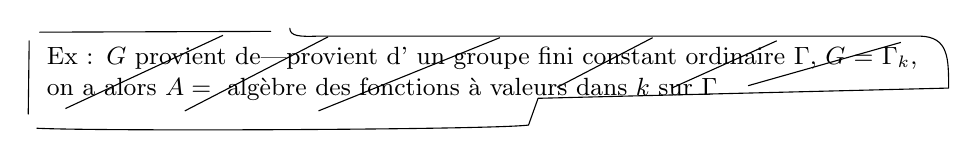
\begin{tikzpicture}[x=\linewidth,y=1cm]
\node[anchor=north west,inner sep=0pt,text width=.92\linewidth,font=\small] at (.025,.02)
 {\deleted{Ex : $G$ \inserted{\unsure{provient de|provient d'}} un groupe fini \deleted{constant} \inserted{ordinaire} $\Gamma$, $G=\Gamma_k$, on a alors $A={}$ algèbre des fonctions \inserted{à valeurs dans $k$} sur $\Gamma$}};
\draw[line cap=round,line join=round] (.018,.21) -- (.26,.22)
 (.28,.26) .. controls (.28,.16) and (.29,.15) .. (.31,.16)
 -- (.94,.16) .. controls (.97,.15) and (.97,-.12) .. (.97,-.50)
 -- (.54,-.63) -- (.53,-.97) .. controls (.49,-1.03) and (.08,-1.05) .. (.015,-1.01)
 (.006,-.83) -- (.007,.10);
\draw (.045,-.76)--(.21,.17) (.17,-.79)--(.32,.15)
 (.31,-.79)--(.50,.14) (.56,-.49)--(.66,.14)
 (.68,-.50)--(.79,.10) (.76,-.47)--(.92,.08);
\end{tikzpicture}}

% @ 14–17
\[
 gg^{-1}=1
\]
\diagram{\begin{tikzcd}[ampersand replacement=\&,column sep=large]
 G \arrow[dr,"{\unsure{\dot p|p|j}}"] \arrow[r,dash,"{\mathrm{id}_G\times\sigma}",to path={-- ++(1.6pt,0pt) -- ++(1.3pt,1.3pt) -- ++(-1.9pt,-2.4pt) -- ++(.7pt,1.1pt) -- (\tikztotarget) \tikztonodes -- ++(0pt,-1.1pt)}] \& G\times G \arrow[r,"{\pi}",dash,to path={-- (\tikztotarget) \tikztonodes -- ++(0pt,-1.3pt)}] \& G \\
 \& e \arrow[ur,"{\varepsilon}"] \&
\end{tikzcd}}
% @ 15 opposite first diagram
\[
 \deleted{A\to A\otimes A}
\]

% @ 18–21
\diagram{\begin{tikzcd}[ampersand replacement=\&,column sep=large]
 x\sigma y \& (x,y) \arrow[l,maps to] \& \\
 A \& A\otimes A \arrow[l] \& A \arrow[l,"{\pi}"] \arrow[dl,"{\varepsilon}"] \\
 \& k \arrow[ul,"p"] \&
\end{tikzcd}}
% @ 18–21 left margin
% margin note written sideways
\margin{\diagram{\rotatebox{90}{\begin{tikzcd}[ampersand replacement=\&,column sep=small,row sep=small,font=\scriptsize]
 \deleted{X\times Y}\;A \arrow[dr,"{\varepsilon}"'] \& A\otimes A \arrow[l] \arrow[d,shift left] \arrow[d,shift right] \& x\otimes y \\
 \& k \& \unsure{\varepsilon(x)\varepsilon(y)|\varepsilon x)\varepsilon y)}
\end{tikzcd}}}}
% archive sheet number: 31
\scanpage{33}
% @ 1
E\uline{xemples de groupes algébriques affines sur} $k$.

% @ 2–8
\diagram{\scriptsize\(\begin{array}{@{}l@{\;}l@{\;}l@{\;}c@{\;}l@{}}
G_m, & G_a, & \mathrm{GL}(n), & \mathrm{O}(Q)\unsure{.}, &
 \text{ss-groupe de }\mathrm{GL}(n)\ \text{invariant des tenseurs}\\[-.5ex]
&&\mathrm{SL}(n)&\begin{array}{c}\cap\\[-.8ex]\mathrm{GL}(n)\end{array}
 &\hfill .\,.\,.\,.\,. \\
&&\mathrm{Tr}(n)&&\\
\unsure{\mathrm{Sp}.|\mathrm{Ex}.}&&\mathrm{Tr}_{\unsure{0|o}}(n)&&\\
\multicolumn{2}{r}{\mathrm{Diag}_0(n)} & \multicolumn{1}{l}{\subset\mathrm{Diag}(n)} &
\multicolumn{2}{l}{\text{immersion de }G_a\text{ dans }\mathbb{G}\unsure{\mathbb{L}|\mathrm{L}}(2)}\\
\multicolumn{2}{c}{\vcenter{\hbox{\tikz[baseline]\node[rotate=90,inner sep=0pt]{\(\unsure{\simeq|\sim}\)};}}} &&&\\
\multicolumn{2}{c}{G_m}&&&
\end{array}\)}

% @ 9
Soit $M$ un $k$-module.
% @ 10–11
\[
 W(M):\unsure{\{|\varepsilon}\ k'\longmapsto M\otimes_k \unsure{k|K}'
 \qquad\text{\parbox{.4\linewidth}{(en fait un $\unsure{\mathcal{O}|\mathscr{O}}_k$-Module, pas seulement un groupe)}}
\]

% @ 11–13
$\cdot$ Pour que ce soit représentable, il faut que $W(M)$ transforme injections $k'\unsure{-|\to} k''$ en injections, donc que $M$ soit p\uline{lat} sur $k$. \deleted{\unsure{So|Si}}

% @ 14–15
Il faut qu'il transforme produits (infinis) d'algèbres en produits
\[
 M\otimes_k\prod k'_i\longrightarrow\prod_i M\otimes_k k'_i
 \qquad\text{bijectif.}
\]

% @ 16–18
\deleted{On voit que ceci} faisant tous les $k'_i$ égaux \unsure{:|à} $k$, on trouve
\[
 M\otimes k^I\xrightarrow{\sim}\deleted{\unsure{\prod_i|\prod}} M^I
\]
% @ 19–21
Et on voit tout de suite que celà implique que $M$ est de type fini, \unsure{donc} \deleted{\unsure{un|une}} quotient d'un libre \deleted{\unsure{fini|f}} \deleted{\unsure{$R\mathrel{-}L$}} \deleted{\unsure{comme|librement}} on a $R\mathrel{-}L\mathrel{-}M\mathrel{-}0$
% @ 22–25
et comme $M$ est plat, \unsure{cel|celà} reste exact par $\otimes_k k^I$, donc $R\otimes k^I\xrightarrow{\sim}R^I$, donc $R$ de type fini, donc $M$ de présentation finie, donc $M$ plat de prés. finie, donc $M$ projectif de t-f. (facteur direct d'un libre)

% @ 26–27
Inversement, si $M$ projectif de t.f. \unsure{i.e.} facteur direct d'un libre $L$\inserted{$\simeq k^{\unsure{n}}$}, par projecteur $p$, on a
% @ 28–29
\[
 \begin{aligned}
 M\otimes_k k'&=\mathrm{Ker}\big((1-p)_{k'}:k'^{n}\to k'^{n}\big)\\
 W(M)&=\mathrm{Ker}\big(\mathbb{E}^{n}\overset{1-p}{\unsure{\relbar|\to}}\mathbb{E}^{n}\big)
 \end{aligned}
\]
% @ 30
c'est repr.

% archive sheet number: 32
\scanpage{34}
% @ 1
\[
 \unsure{\mathbb{V}|V}(M)=\operatorname{Hom}_{k\text{-mod}}(M,k')
 =\operatorname{Hom}_{k'\text{-mod}}(M\otimes_k k',k')
\]
% @ 2
\uline{\unsure{tjrs|tjrs.}} représentable par
\[
 \operatorname{Sym}^{*}_k(M)=\sum_{n\geq0}\operatorname{Sym}^{n}_k(M)
\]

% @ 3–6
\[
\resizebox{\linewidth}{!}{\(\displaystyle\begin{aligned}
\Big[\, V(M)\times W(M)&\longrightarrow\deleted{\unsure{\mathbb{E}|E}}\unsure{\mathcal{O}|\mathscr{O}}_k=W(k)
&
\mathbb{V}(M)&\xrightarrow{\sim}
 \underbrace{\underline{\operatorname{Hom}}_{\mathcal{O}_k}
 (W(M),\deleted{\unsure{\mathcal{O}_k|\mathbb E_k}}W(k))}\\
&\unsure{V|\surd}&&
 k'\longmapsto\operatorname{Hom}\big(
  \overbrace{W(M)_{k'}}^{\inserted{\simeq\,W(\unsure{M_{k'}|M})}},
  \deleted{\unsure{\mathcal{O}_{k'}|\mathcal{O}_{k}}}W(k')\big)\\
&&&\hspace{3.7em}\vcenter{\hbox{\tikz[baseline]\node[rotate=90,inner sep=0pt]{\(=\)};}}\\[-.5ex]
&&&\operatorname{Hom}_{k'}(M_{k'},k')=\operatorname{Hom}_k(M,k'\unsure{)}
\end{aligned}\)}
\]

% @ 6–7
\unsure{Or|or}\quad $M\longmapsto W(M)$
\[
 \operatorname{Mod}(k)\longmapsto\operatorname{Mod}(\mathcal{O}_k)
 \qquad\text{est pl\uline{einement fidèle}.}
\]
% @ 8–10
\figure{\footnotesize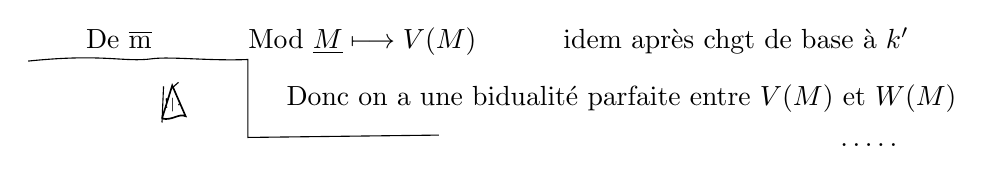
\begin{tikzpicture}[x=\linewidth,y=1cm]
\node[anchor=base west,inner sep=0pt] at (.06,1.18) {De $\overline{\mathrm{m}}$};
\node[anchor=base west,inner sep=0pt] at (.23,1.18) {\deleted{Mod} $\underline{M}\longmapsto V(M)$};
\node[anchor=base west,inner sep=0pt] at (.56,1.18) {idem après chgt de base à $k'$};
\draw (0,1.02) .. controls (.08,1.12) and (.10,1.00) .. (.13,1.05)
 .. controls (.15,1.08) and (.19,1.02) .. (.23,1.04)
 -- (.23,.05) -- (.43,.08);
\begin{scope}[shift={(.15,.45)},x=1cm,y=1cm]
 \draw[line width=.6pt] (-.12,-.16) -- (.01,.26) -- (.18,-.13)
  .. controls (.09,-.09) and (.01,-.19) .. (-.12,-.16);
 \draw (-.10,.25) -- (-.12,-.21) (.01,.23) -- (.09,.30);
 \node[inner sep=0pt] at (.02,.01) {\tiny\(\unsure{!|\cdot}\)};
\end{scope}
\node[anchor=base west,inner sep=0pt] at (.27,.46)
 {Donc on a une bidualité parfaite entre $V(M)$ et $W(M)$};
\node[anchor=base west,inner sep=0pt] at (.85,-.07) {.\,.\,.\,.\,.};
\end{tikzpicture}}

% @ 11
\[
 \underline{\operatorname{Aut}}_{\mathcal{O}}(M)\subset
 \underline{\operatorname{End}}_{\mathcal{O}}(M)
 \qquad\text{représentable si $M$ est proj., \unsure{t f.|t.f.}}
\]

% @ 12
\noindent\hspace{.05\linewidth}\rule{.31\linewidth}{.4pt}

% @ 13
\[
 \mu_n,\ D(\unsure{\vcenter{\hbox{\tikz[x=1ex,y=1ex]{\draw[line width=.12ex,line cap=round,line join=round] (0,0)--(.04,1.07)--(.94,1.09)--(.91,.6);\fill (.30,.82) circle[radius=.055ex];}}}|\Gamma|\Pi})\quad .\,.\,.
\]

% archive sheet number: 33
